% Set the author and title of the compiled pdf
\hypersetup{
	pdftitle = {\Title},
	pdfauthor = {\Author}
}

\section{Course intro}

A smartphone is a mobile phone running a mobile operating system, with advanced
capabilities with regard to computing power and connectivity. They are much more
advanced than traditional feature phones, and have lots of features, including
cameras, multimedia functionality, GPS, touch screens etc.

There are three main mobile operating systems in use today:

\begin{description}
  \item \textbf{Android}\\
  	Founded in 2003 by Andy Rubin and backed by Google. It's mostly free and
  	open source, and holds a very strong position in the market.
  \item \textbf{iOS}\\
  	Introduced in 2007 by Apple, this is a closed source operating system. The
  	first iOS phones were very groundbreaking in terms of their technology, and
  	were the first to feature touch screens, which are now ubiquitous in the
  	market.

\marginpar{Blackberry, Symbian, Palm OS etc could be listed here too.}

  \item \textbf{Windows Phone}\\
    Version seven was released in 2010, previous versions were terrible (imho).
\end{description}

\subsection{What's in a smartphone?}

Modern smartphones are jam packed with technology, containing cameras,
multimedia, GPS, high resolution touch screens, motion sensors, bluetooth, RFID,
NFC and even more stuff besides. They let you talk over multiple different
networks (2G, 3G, 4G etc), and access data using the same methods.

Of course, the millions of apps available for them is also a massive attraction.

Smartphones Operating Systems need to be very advanced in order to step up to
the tasks required of them by users. They need to be multitasking, to run lots
of different apps, and interface with the typical hardware a normal computer
might use (DMA, standard (ish) input devices etc). However, they also need to
have real-time elements in, since they must be able to drive sound, IO, radio
communications, digital signal processing etc

% Lecture two
\section{Signals in mobile systems}

Signals such as speech and music arrive at the device as physical, analogue
quantities that vary in a continuous manner over time. If we plot a graph of
voltage over time, then we get a waveform for that signal. We can convert
analogue signals to \textit{discrete time signals} by sampling them at set
intervals (discrete points in time). This produces a list of numbers from
$-\inf$ to $\inf$.

\subsection{Generating waves}

In order to create a wave with a period of $T$ seconds, you can use the formula:

\[
  y = sin(\frac{2\pi x}{T})
\]

Of course, since $f = \frac{1}{T}$, the frequency of the wave is the reciprocal
of the time period.

\subsection{Sampling waves}

We can work out the frequency of a wave, by finding how many complete cycles it
undergoes in one thousand samples, and multiplying that by the sample rate. For
example, if a wave has ten cycles from $1000$ samples at $30,000Hz$, then its
frequency will by $\frac{10}{1000} \times 30,000 = 300Hz$. This is visible in
Figure~\ref{discrete-signal}.

\begin{figure}
  \centering
  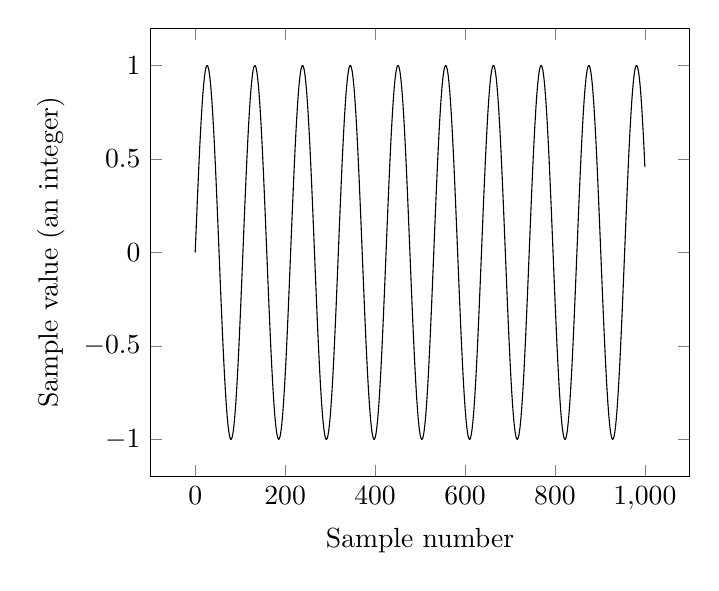
\begin{tikzpicture}
    \begin{axis}[%
      domain = 0:1000,
      samples = 1000,
      xlabel={Sample number},
      ylabel={Sample value (an integer)}]
      \addplot[black,thin] {sin(x * pi * (1080/1000))};
    \end{axis}
  \end{tikzpicture}
  \label{discrete-signal}
  \caption{1000 samples of an analogue sin wave of frequency $300Hz$ sampled at
  $30,000$Hz.}
\end{figure} 

Not all waves are so easy to analyse, rarely will a wave be at just one
frequency, instead, they are usually `noisy' and will be composed of many waves
added together. Many waves (that aren't just noise) will have a discernible
frequency that you can extract. The `extra' waves on top of this frequency
aren't necessarily bad, they might add harmonics, or texture to a sound.

\subsubsection{Quantisation}

When we've sampled a wave, if we leave all of our readings as floating point
numbers, then we could be using a lot of space to store each sample. We could
slightly reduce the quality of our sound by \textit{quantising} it. This is when
you map the continuous values onto a range of integers, where the range of
integers spans a power of two (so you can use as few bits as possible).

You can see that the third wave in Figure~\ref{quantised-wave} has been
quantised into five integers, since there are five discrete values in the
waveform ($0,1,2,3,4$) (requiring four bits), and there will be an extra bit to
indicate the sign. If whoever made the diagram was trying to be as efficient as
possible, they might have had either one less value (so that the numbers could
be represented in three bits), or made full use of the four bits for the value,
and used values from $0-7$.

\begin{figure}[H]
  \centering
  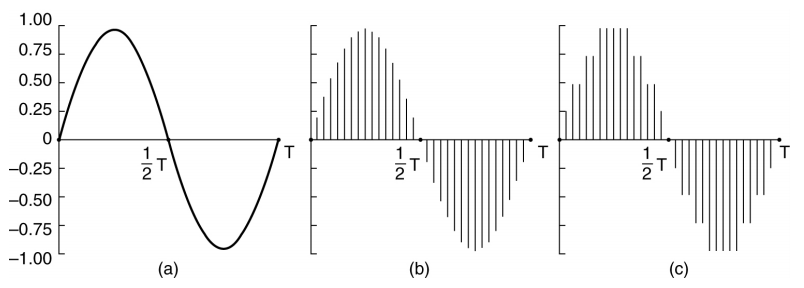
\includegraphics[width=\textwidth]{images/quantised-wave}
  \caption{An analogue wave (a), after its sampled (b), and once it's been quantised (c)}
  \label{quantised-wave}
\end{figure}

Quantisation produces noise (known as quantisation noise), since errors are
introduced in the process. If there are many bits per sample (e.g. 16), then
this error will be small, but if you only used say, five bits, then the error
would be noticeable. As a consequence of this, we have to work a trade-off
between storage capacity or bandwidth and quality.

\subsubsection{The Sampling Theorem}

\marginpar{Also known as \textit{Nyquist criterion}.}

The Sampling Theorem states that if a signal has all of its spectral energy
below $B$Hz, and is sampled at $F$Hz, where $F \geq 2B$, then it can be
reconstructed \textit{exactly} from the samples and nothing is lost.

In other words, if you are sampling a signal at \textit{less than half} of the
maximum frequency of the signal, then you won't be able to fully reconstruct the
signal from the samples, and you will get distortion.

Since music is usually sampled at $44.1$\si{\kilo\hertz}, we can accurately sample music with
frequencies up to around $22$\si{\kilo\hertz}. Speech rarely has frequencies above $3.4$\si{\kilo\hertz},
so the sample rate for it can be much lower, as we will see later on in the
course.

\subsubsection{Aliasing}

If we sample at less than twice the frequency of the wave, then we will get
distortion, known as aliasing. The first lab on this course relates to aliasing.
Even if we don't want frequencies higher than half our sample rate, we need to
filter them out anyway, since otherwise, we will get aliasing when we sample
them.

To be precise, if a wave of frequency $f$ is sampled at a frequency of below
$2f$ (lets call this $F$, then the sampled output will be a wave of frequency $F
- f$.

For example, if we sample a $6\si{\kilo\hertz}$ wave at a frequency of $10\si{\kilo\hertz}$, when we will
get a wave of frequency $10-6 = 4\si{\kilo\hertz}$.

This is bad, because if you have harmonics in a musical note that are higher
than half the sampling frequency, then these harmonics will be out of tune post
sampling, and will go down when it's supposed to go up.

It may be hard to work out exactly why aliasing occurs, but
Figure~\ref{aliasing}, showing a $6\si{\kilo\hertz}$ wave sampled at $8\si{\kilo\hertz}$ makes it easier
to see:

\begin{figure}[H]
  \centering
  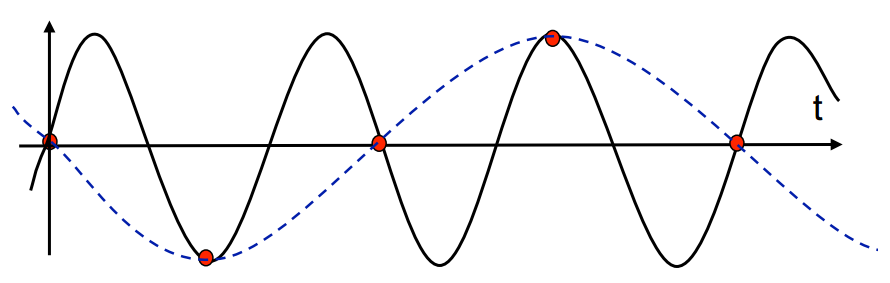
\includegraphics[width=\textwidth]{images/aliasing}
  \caption{A $6\si{\kilo\hertz}$ wave sampled at $8\si{\kilo\hertz}$ has a post-sampling frequency of 
  $2\si{\kilo\hertz}$}
  \label{aliasing}
\end{figure}

% Slide 15 of lecture 2

\section{Storing signals}

Signals are stored in many different ways. One `easy' format, is the
\texttt{.wav} format. It is just a list of binary numbers, each representing a
single value of the wave at a discrete time.

% TODO: More formats, encoding etc
